\documentclass[letterpaper, 10pt,titlepage]{article}

\usepackage[utf8]{inputenc}
\usepackage [english]{babel}
\usepackage{graphicx}
\graphicspath{}
\newcommand\tab[1][1cm]{\hspace*{#1}}
\setlength{\parindent}{0em}
\setlength{\parskip}{1em}
\usepackage[letterpaper, margin=0.75in]{geometry}
\usepackage{balance}
\usepackage{hyperref}
\usepackage{minted}
\hypersetup{
  colorlinks = true,
  linkcolor  = black
}

\setcounter{secnumdepth}{4}
\def\name{Group 48}

\graphicspath{ {images/}}

\hypersetup{
  colorlinks = true,
  urlcolor = black,
  pdfauthor = {\name},
  pdfkeywords = {Spring Midterm Progress Report},
  pdftitle = {Capstone Project},
  pdfsubject = {Capstone Project},
  pdfpagemode = UseNone
}



\begin{document}

\begin{titlepage}
\begin{center}
    \Huge
    \textbf{Winter Progress Report}\\
    \textbf{Capstone Project}\\
    \vspace{1.0cm}
    \large
    Author: Xiaoli Sun\\
    Client: David Vasquez\\
    \vspace{1.5cm}
    \large
    Instructor: D. Kevin McGrath, Kirsten Winters\\

    \large
    CS 462, Winter 2018, Oregon State University\\    

    \vspace{3.2cm}

    \large
    \underline{Abstract}\\
    \vspace{0.3cm}
    \end{center}
    \large

    \tab For the Campus Event Mobile Application program, the client David Vasquez want to make life more convenient for each students, instructors or even residents live in Corvallis since there are lots of events happen everyday. A great mobile application is useful for every user and improve the quality of life. The mobile application will be developed in two forms: one developed for the Android mobile platform, and the other developed for the iOS mobile development. For the ease of development, these two forms of the mobile application will be developed with a framework called React Native which support cross platform development, they will be using the same methods of providing campus events to users. The mobile application will display current events and group events by loading data from MySQL database. In addition, the mobile application will allow users discover different events from different sections, follow and unfollow events, and edit user profile. 
    \vspace{0.8cm}
    \vfill
    
\begin{center}    
    Mar 17, 2018

\end{center}
\end{titlepage}


\tableofcontents
\newpage

\section{Xiaoli Sun's section}
\subsection{Purpose and Goals}
Various organization holds multiple events every year in Oregon State University. To let the Corvallis community more involved, Evently will display multiple group events to the public. The mobile application will provide user interact calendar as a view to keep track of all the events that they want to see. Users will also available to find new events according to different categories. Moreover, users have access to discover all groups that they interested and can participate with. The mobile application will have secure login to further protect user information. The application is developed under React Native. \\ \\

\subsection{Current status}
Currently, I finished implementing secure login of the project and also changed file structure of whole project to make it looks more logically and clearly. I found a tutorial on Medium.com for how to build a React Native application using Firebase. To implement the secure login, we plan to change from using OSU OAuth 2 API to use Firebase Google login and email/password login. First of all, I created two new applications in Firebase console. One for Android and one for iOS. The package name was set to host.exp.exponenet because we used Expo API in the application. After applications were created, email/password and Google login should be enabled in SIGN-IN METHOD tab. After all preparations are set up, I began to implement this feature in our project. First of all, I used following react native packages for implementing secure login: Redux is used for managing the application's state. React-Redux is used to connect our application to Redux store. Redux Thunk allow me to write action creators. React-native-router-flux is used to manage navigation of the application. React-Native-Redux-Listener is used to detect network changes. Axios is a HTTP client for making calls to API. The back end contains several JavaScript files which were used to store Firebase application configuration information, create an instance of the Firebase SDK by using the stored configuration information and update the state of the application. constants.js is used to store Firebase configuration information. In firebase.js, an instance of the Firebase SDK is created by using Firebase configuration information. In rootReducer.js, combineReducers function is used to merge reducer from auth and home directory together. Redux store is created in store.js. Several functions including register, login that interact with Firebase API are created in api.js. Functions that created in actions.js are used to call correct API functions. The front end contains files for the UI of login and register screen. The styles like fonts and color was also set up in front end. validate.js is used to check if the username, email or password meets the requirement or not. AuthTextInput.js creates a view contains a label and TextInput. Form.js contains a component that create a TextInput for each field. Splash.js notify users the app is loading and also checks whether a user is logged in or not. Welcome.js create a main login scene that display user two buttons, one for email/password login and one for Google login. Register.js use form component and calls register function. If the function return successfully, onSuccess function is called and the application is advanced to CompleteProfile screen. Login function from action.js is called in login.js and then user will be navigates to the main screen of the application. ForgetPassword.js allow user reset password. CompleteProfile.js calls createUser function and store user name to Firebase realtime database. After all screen above were implemented, I wrapped up these screens to route.js by using react-native-router-flux. Finally, I used Expo API in app.js to load font and icons.\\ \\

\subsection{What's left}
Since there's only one week away from code freeze, not many tasks is left. My task is implementing secure login and notification push. Because we haven't set up the database, I can't implement notification push until database is set up. Our client David already allow us to set notification push as a stretch goal. The main task that we need to finish during the next week is to create data in Firebase realtime database. It's too late for us to decide to use Firebase realtime database because secure login is not easy to implement and I just implemented secure login using Firebase this term. Firebase realtime databse  use NoSQL and none of us learned it before. We will try our hard to learn NoSQL and finish our project.\\ \\

\subsection{Problems}
The most difficult part during implementing secure login is to understand how to keep or update the state of application. The next problem is that the header bar in Event page can't display correctly. When I hide child navbar in stack, the parent navbar would also be hidden. I spent a lot of time searching online for this problem and final found that this problem is caused by react-navigation and react-native-router-flux failed to support hiding child navbar without hiding parent navbar. There's no answer to solve this problem if using react-native-router-flux.\\ \\

\subsection{JavaScript code}
\subsubsection{JavaScript code for Welcome.js}
\begin{minted}{javascript}
import React from 'react';
import {Text, View, TouchableOpacity, Image} from 'react-native';

import { Google } from 'expo';
import {Button, SocialIcon, Divider} from 'react-native-elements'
import {Actions} from 'react-native-router-flux'
import {connect} from 'react-redux';

import {actions as auth, constants as c } from "../../index"
const { signInWithGoogle } = auth;

import styles from "./styles"

class Welcome extends React.Component {
    constructor() {
        super();
        this.state = {}

        this.onSuccess = this.onSuccess.bind(this);
        this.onError = this.onError.bind(this);
        this.onSignInWithGoogle = this.onSignInWithGoogle.bind(this);
    }

    async onSignInWithGoogle(){
        try{
            const result = await Google.logInAsync({
                androidClientId: c.GOOGLE_SIGN_IN_ANDROID_ID,
                iosClientId: c.GOOGLE_SIGN_IN_IOS_ID,
                scopes: ['profile', 'email'],
            });

            if(result.type === 'success'){
                this.props.signInWithGoogle(result.idToken, result.accessToken, this.onSuccess, this.onError);
            }
        }catch(e) {
            return {error: true};
        }
    }

    onSuccess({ exists, user}) {
        if (exists) Actions.Main();
        else Actions.CompleteProfile({ user });
    }

    onError(error) {
        alert(error.message);
    }

    render() {
        return (
            <View style={styles.container}>
                <View style={styles.topContainer}>
                    <Image style={styles.image} source={{uri: ""}}/>
                    <Text style={styles.title}>Welcome to Community Events!</Text>
                </View>

                <View style={styles.bottomContainer}>
                    <View style={[styles.buttonContainer]}>
                        <SocialIcon
                            raised
                            button
                            type='google'
                            title='SIGN UP WITH GOOGLE'
                            iconSize={19}
                            style={[styles.containerView, styles.socialButton]}
                            fontStyle={styles.buttonText}
                            onPress={this.onSignInWithGoogle}/>

                        <View style={styles.orContainer}>
                            <Divider style={styles.divider}/>
                            <Text style={styles.orText}>
                                Or
                            </Text>
                        </View>

                        <Button
                            raised
                            borderRadius={4}
                            title={'SIGN UP WITH E-MAIL'}
                            containerViewStyle={[styles.containerView]}
                            buttonStyle={[styles.button]}
                            textStyle={styles.buttonText}
                            onPress={Actions.Register}/>
                    </View>
                    <View style={styles.bottom}>
                        <Text style={styles.bottomText}>
                            Already have an account?
                        </Text>

                        <TouchableOpacity onPress={Actions.Login}>
                            <Text style={styles.signInText}>
                                Sign in
                            </Text>
                        </TouchableOpacity>
                    </View>
                </View>

            </View>
        );
    }
}


export default connect(null, { signInWithGoogle })(Welcome);

\end{minted}

\section{Sung Kim}
\subsection{Purpose and Goals}

Our goal should still be the same, produce an application that will meet the needs of our client David Vasquez. To do this we will develop an application that will run on both Android and IOS, Evently will also be simple and easy to use. Although it is currently an application made for the Corvallis community, there is room for it to grow. David has mentioned the possibility for the application to reach other college towns so that no one will have to miss an event again. As for my personal goals, I want to make sure the team has nothing to worry about in terms of getting ready for Expo.

\subsection{Current Status}

As of now, the development of the application has been going well, Xiaoli was able to implement a login page through Google's Cloud Platform service, Firebase. With this, we were able to implement a secure login on our mobile application. There was some issues after implementing this, which will be mentioned later, but for now I will go into the pros for switching. With the Google Firebase Cloud service, it gave us a centralized database to hold all of our data. This was a one of our biggest issues in the past since the group had to use WAMP server to create a local SQL database. This was an issue itself because the database was local, meaning you would only be able to access the data from the computer the server was running on. Firebase also provides us with a bunch of tools for our application such as crash reports and many other performance monitoring tools. The best part of using this service is the fact that it's free to use, unless you want to upgrade to a more premium package. Along with learning how to use this new tool, I have been getting everyone ready for the upcoming expo. I have been the main source of contact between my team and David, while taking care of all the paperwork for the team. Sadly, David will most likely not be able to attend the engineering expo, due being busy with work and school, so he will be with us in spirit. 

\subsection{What's Left}

What's left for our project is cleaning up the application, connecting the new database and showing off our project at the expo. When I say cleaning, we just need to keep making the application look prettier. It's still a little rough around the edges, so with a little bit more work it'll look a lot better. Connecting our application to the new database might take a little longer since the entire team has no experience with a NoSQL database. A majority of the application is already there, so once we finish connecting the database we should be close to finishing. As showing off our project, the team is looking forward to seeing all the other projects and displaying ours to the community. 

\subsection{Problems}

The biggest issue I currently see is the fact that our team moved from using MySQL to the Firebase NoSQL database. We are learning while using the tools to display our information, but I feel the this is a minor disturbance versus the benefits this tool will bring us in the long run. One more issue that bothers me a little bit, but doesn't affect the progress of our application, is that we're still using dummy data. This has been mentioned in previous progress reports and is probably the smallest thing to worry about, but still bothers me a little bit. 

\section{Zijian Huang}
\subsection{Purpose and Goals}
There are many events happened in Oregon State University every week. The app Evently which implement by group 48 is try to put all of the events which will happened in OSU into this application, for help the residences who live in Corvallis Community or campus students get all the events information quickly and accurately. This mobile application could provide all of different category of events, and users can choose their favorite category and follow them. Also, the application have the calender which show up all of the events date to help users to track the events they want to go. This application also provide the personal account function which means users can have their own account and personal information in this app. 

\subsection{Current status}
I take part of the follow page. In the last term I face the problem which is the Json could not push more than one table insert at last week. After that I searched a lot to fix this problem. It took a while and now I think the only thing on the following part is the database. Since our group could test the Android and IOS platform right now and the Android platform look pretty good at this time just some small part need to be fixed, it is not a big problem with the IOS platform. For the application, right now the secure login is almost finished, just something need to be fixed. Also. we need a notification push function which could help user to get information they want in time. But the notification push is the extension target which our client David allowed, so if we have left time to achieve this functionality, we need to use some mainstream function on firebase to implement it. For the follow page, since we don't have the OSU events database to use, we just use some dummy data to make tables and insert to the application. It is the only way to achieve a complete page show up but the data will not provide all of the events since we could not get all the events data promptly. Moreover, since all the teammates have no experiences for NoSQL using, it is probably a difficult progress for us as well. 

\subsection{What's left}
For the left part, since we have just one week to finish our whole project, we need to hurry up the implementation, including find bugs and debugging. For me, the follow page should be completely done, it means all the data table insert should be detailed and reasonable. Also, because the testing of IOS platform should be doing on my computer, it is part of my job to do that. I found the size of interface have some trouble on IOS platform during the test. The bottom of the application have a blank which could be caused by the react native code . Since the react native implementation was on the other computer which is based on implement Android platform. The Android platform application have some buttons on the bottom which could make the blank on the IOS platform. I will try to eliminate that with teammate and make the interface of the IOS platform looks better. Moreover, preparing the EXPO is the thing we should to do before it coming up, we hope on that day, my teammates and I could have a great status to face the visitors and their questions. As above, that's the what I and our team left.

\subsection{Problems}
For the problems, the most difficult part is the database which we have could not make the application be a useful tool to help users. Although the dummy data could work and make the pages be completed, but it could not for real using because we need to get the data of events after OSU update the data and put them insert our database at all time. It is not a feasible way for the application in the future. Also, because of the devision of work, some of the files of code will replace others. It is a problem which is not difficult to solve but very inefficient. To solve that problem, my teammates and I need to rearrange the code part and make sure all the part of work could be combined and perfectly run.

\section{Conclusion}
Overall most functionality of the mobile application is already implemented. Our progress has already showed some results. The user interface and backend of the mobile application all are coming along nicely. In next term, we will certainly implement secure login to the application. After all functionality is implemented, we will attend expo and show our projects to visitors.\\

\subsection{Screenshots}
\newpage
\includegraphics[width=\textwidth, height=\textheight]{welcome.eps}
\newpage
\includegraphics[width=\textwidth, height=\textheight]{signup.eps}
\newpage
\includegraphics[width=\textwidth, height=\textheight]{login.eps}
\newpage
\includegraphics[width=\textwidth, height=\textheight]{forgetpassword.eps}
\newpage
\includegraphics[width=\textwidth, height=\textheight]{completeprofile.eps}
\newpage
\includegraphics[width=\textwidth, height=\textheight]{signup.eps}
\newpage
\newpage
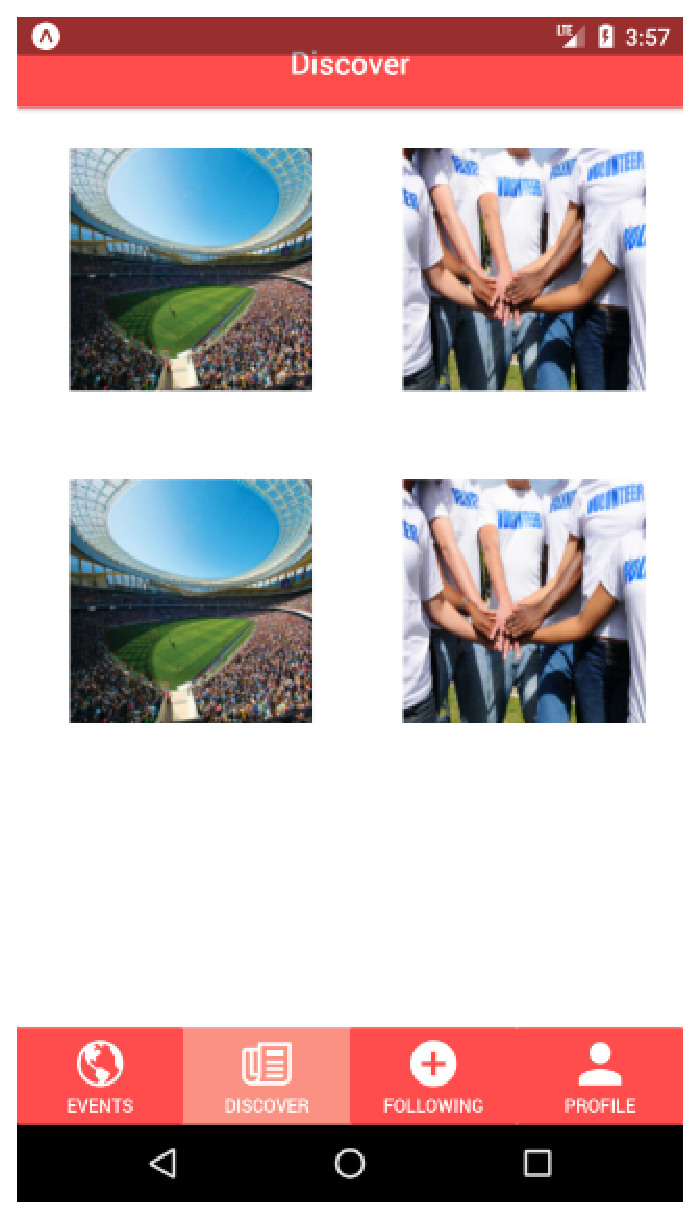
\includegraphics[width=\textwidth, height=\textheight]{Discover_Screen.eps}




\end{document}
